% Options for packages loaded elsewhere
\PassOptionsToPackage{unicode}{hyperref}
\PassOptionsToPackage{hyphens}{url}
\PassOptionsToPackage{dvipsnames,svgnames,x11names}{xcolor}
%
\documentclass[
  ignorenonframetext,
]{beamer}
\usepackage{pgfpages}
\setbeamertemplate{caption}[numbered]
\setbeamertemplate{caption label separator}{: }
\setbeamercolor{caption name}{fg=normal text.fg}
\beamertemplatenavigationsymbolsempty
% Prevent slide breaks in the middle of a paragraph
\widowpenalties 1 10000
\raggedbottom

\usepackage{amsmath,amssymb}
\usepackage{iftex}
\ifPDFTeX
  \usepackage[T1]{fontenc}
  \usepackage[utf8]{inputenc}
  \usepackage{textcomp} % provide euro and other symbols
\else % if luatex or xetex
  \usepackage{unicode-math}
  \defaultfontfeatures{Scale=MatchLowercase}
  \defaultfontfeatures[\rmfamily]{Ligatures=TeX,Scale=1}
\fi
\usepackage{lmodern}
\usetheme[]{AnnArbor}
\usecolortheme{dolphin}
\usefonttheme{structurebold}
\ifPDFTeX\else  
    % xetex/luatex font selection
\fi
% Use upquote if available, for straight quotes in verbatim environments
\IfFileExists{upquote.sty}{\usepackage{upquote}}{}
\IfFileExists{microtype.sty}{% use microtype if available
  \usepackage[]{microtype}
  \UseMicrotypeSet[protrusion]{basicmath} % disable protrusion for tt fonts
}{}
\makeatletter
\@ifundefined{KOMAClassName}{% if non-KOMA class
  \IfFileExists{parskip.sty}{%
    \usepackage{parskip}
  }{% else
    \setlength{\parindent}{0pt}
    \setlength{\parskip}{6pt plus 2pt minus 1pt}}
}{% if KOMA class
  \KOMAoptions{parskip=half}}
\makeatother
\usepackage{xcolor}
\newif\ifbibliography
\setlength{\emergencystretch}{3em} % prevent overfull lines
\setcounter{secnumdepth}{-\maxdimen} % remove section numbering


\providecommand{\tightlist}{%
  \setlength{\itemsep}{0pt}\setlength{\parskip}{0pt}}\usepackage{longtable,booktabs,array}
\usepackage{calc} % for calculating minipage widths
\usepackage{caption}
% Make caption package work with longtable
\makeatletter
\def\fnum@table{\tablename~\thetable}
\makeatother
\usepackage{graphicx}
\makeatletter
\def\maxwidth{\ifdim\Gin@nat@width>\linewidth\linewidth\else\Gin@nat@width\fi}
\def\maxheight{\ifdim\Gin@nat@height>\textheight\textheight\else\Gin@nat@height\fi}
\makeatother
% Scale images if necessary, so that they will not overflow the page
% margins by default, and it is still possible to overwrite the defaults
% using explicit options in \includegraphics[width, height, ...]{}
\setkeys{Gin}{width=\maxwidth,height=\maxheight,keepaspectratio}
% Set default figure placement to htbp
\makeatletter
\def\fps@figure{htbp}
\makeatother
% definitions for citeproc citations
\NewDocumentCommand\citeproctext{}{}
\NewDocumentCommand\citeproc{mm}{%
  \begingroup\def\citeproctext{#2}\cite{#1}\endgroup}
\makeatletter
 % allow citations to break across lines
 \let\@cite@ofmt\@firstofone
 % avoid brackets around text for \cite:
 \def\@biblabel#1{}
 \def\@cite#1#2{{#1\if@tempswa , #2\fi}}
\makeatother
\newlength{\cslhangindent}
\setlength{\cslhangindent}{1.5em}
\newlength{\csllabelwidth}
\setlength{\csllabelwidth}{3em}
\newenvironment{CSLReferences}[2] % #1 hanging-indent, #2 entry-spacing
 {\begin{list}{}{%
  \setlength{\itemindent}{0pt}
  \setlength{\leftmargin}{0pt}
  \setlength{\parsep}{0pt}
  % turn on hanging indent if param 1 is 1
  \ifodd #1
   \setlength{\leftmargin}{\cslhangindent}
   \setlength{\itemindent}{-1\cslhangindent}
  \fi
  % set entry spacing
  \setlength{\itemsep}{#2\baselineskip}}}
 {\end{list}}
\usepackage{calc}
\newcommand{\CSLBlock}[1]{\hfill\break\parbox[t]{\linewidth}{\strut\ignorespaces#1\strut}}
\newcommand{\CSLLeftMargin}[1]{\parbox[t]{\csllabelwidth}{\strut#1\strut}}
\newcommand{\CSLRightInline}[1]{\parbox[t]{\linewidth - \csllabelwidth}{\strut#1\strut}}
\newcommand{\CSLIndent}[1]{\hspace{\cslhangindent}#1}


% logo
\titlegraphic{
\includegraphics[width=4cm]{000_logos/logo-blue-vertical}}
\logo{\ifnum\thepage>1
\includegraphics[width=0.5cm]{000_logos/logo-blue-vertical}\fi}

% UMNG: Manual de image institucional

% Colors

% Umng
\definecolor{yellow}{HTML}{fdc600}
\definecolor{red}{HTML}{ee2a24}

% Estudios a Distancia
\definecolor{blue1}{HTML}{12245b}
\definecolor{blue2}{HTML}{767ca6}
\definecolor{blue3}{HTML}{cad2ec}

% Modify items
\setbeamercolor{palette primary}{bg=blue3}
\setbeamercolor{palette tertiary}{bg=blue1}
\setbeamercolor{frametitle}{bg=yellow}

% Hyperlinks
\hypersetup{
  linkcolor=red,
  citecolor=red
}

\makeatletter
\@ifpackageloaded{caption}{}{\usepackage{caption}}
\AtBeginDocument{%
\ifdefined\contentsname
  \renewcommand*\contentsname{Table of contents}
\else
  \newcommand\contentsname{Table of contents}
\fi
\ifdefined\listfigurename
  \renewcommand*\listfigurename{List of Figures}
\else
  \newcommand\listfigurename{List of Figures}
\fi
\ifdefined\listtablename
  \renewcommand*\listtablename{List of Tables}
\else
  \newcommand\listtablename{List of Tables}
\fi
\ifdefined\figurename
  \renewcommand*\figurename{Figure}
\else
  \newcommand\figurename{Figure}
\fi
\ifdefined\tablename
  \renewcommand*\tablename{Table}
\else
  \newcommand\tablename{Table}
\fi
}
\@ifpackageloaded{float}{}{\usepackage{float}}
\floatstyle{ruled}
\@ifundefined{c@chapter}{\newfloat{codelisting}{h}{lop}}{\newfloat{codelisting}{h}{lop}[chapter]}
\floatname{codelisting}{Listing}
\newcommand*\listoflistings{\listof{codelisting}{List of Listings}}
\makeatother
\makeatletter
\makeatother
\makeatletter
\@ifpackageloaded{caption}{}{\usepackage{caption}}
\@ifpackageloaded{subcaption}{}{\usepackage{subcaption}}
\makeatother

\ifLuaTeX
\usepackage[bidi=basic]{babel}
\else
\usepackage[bidi=default]{babel}
\fi
\babelprovide[main,import]{english}
% get rid of language-specific shorthands (see #6817):
\let\LanguageShortHands\languageshorthands
\def\languageshorthands#1{}
\ifLuaTeX
  \usepackage{selnolig}  % disable illegal ligatures
\fi
\usepackage{bookmark}

\IfFileExists{xurl.sty}{\usepackage{xurl}}{} % add URL line breaks if available
\urlstyle{same} % disable monospaced font for URLs
\hypersetup{
  pdftitle={Labor Market},
  pdfauthor={Luis Francisco Gómez López},
  pdflang={en},
  colorlinks=true,
  linkcolor={Maroon},
  filecolor={Maroon},
  citecolor={Blue},
  urlcolor={Blue},
  pdfcreator={LaTeX via pandoc}}


\title{Labor Market}
\author{Luis Francisco Gómez López}
\date{2024-07-17}
\institute{FAEDIS}

\begin{document}
\frame{\titlepage}

\renewcommand*\contentsname{Table of contents}
\begin{frame}[allowframebreaks]
  \frametitle{Table of contents}
  \tableofcontents[hideallsubsections]
\end{frame}

\section{Please Read Me}\label{please-read-me}

\begin{frame}{}
\phantomsection\label{section}
\begin{itemize}
\item
  Check the message \textbf{Welcome greeting} published in the News
  Bulletin Board.
\item
  Dear student please edit your profile uploading a photo where your
  face is clearly visible.
\item
  The purpose of the virtual meetings is to answer questions and not to
  make a summary of the study material.
\item
  This presentation is based on
  (\citeproc{ref-cardenas_introduccion_2020}{Cardenas 2020, chap. 9})
\end{itemize}
\end{frame}

\section{Purpose}\label{purpose}

\begin{frame}{}
\phantomsection\label{section-1}
Examine the evolution and characteristics of the supply and demand of
labor in Colombia
\end{frame}

\section{Labor classification of the
population}\label{labor-classification-of-the-population}

\begin{frame}{}
\phantomsection\label{section-2}
\begin{itemize}
\item
  To understand the indicators of the labor market from an economic
  perspective, it is necessary to classify the population from a labor
  point of view. Initially, the total population of a territory could be
  included but in practice the \textbf{Total Population (TP)} that is
  included \textbf{doesn't} cover
  (\citeproc{ref-hussmanns_surveys_1990}{Hussmanns, Mehran, and Varmā
  1990, chap. 2}):

  \begin{itemize}
  \item
    Members of the armed forces because this information is considered
    secret or because it is not easy to obtain information when its
    members are in barracks and military areas.
  \item
    Residents in institutions such as people who are not part of the
    military forces but reside in military facilities, residents of
    penal or correctional centers and hospital residents.
  \end{itemize}
\item
  In that sense, the \textbf{Total Population (TP)} covers the
  non-institutional civilian population residing in households.
\end{itemize}
\end{frame}

\begin{frame}{}
\phantomsection\label{section-3}
\begin{figure}

\centering{

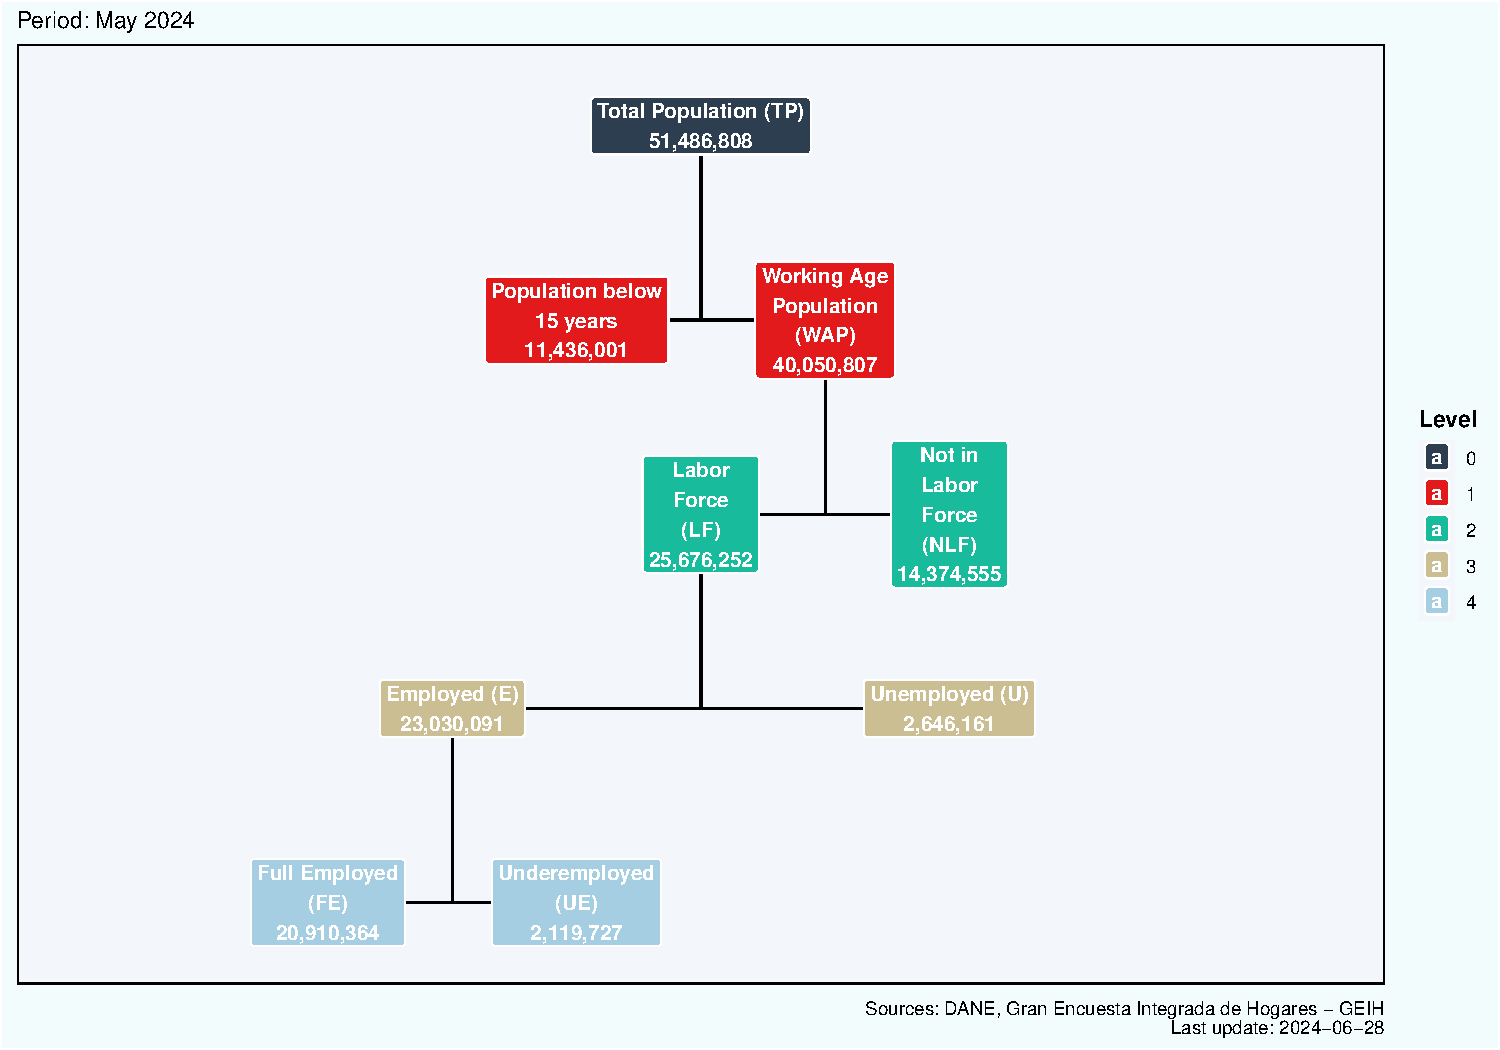
\includegraphics[width=0.85\textwidth,height=\textheight]{009_labor_market_files/figure-beamer/fig-labor-classification-col-1.pdf}

}

\caption{\label{fig-labor-classification-col}Labor classification of the
population in Colombia}

\end{figure}%
\end{frame}

\section{Labor market indicators}\label{labor-market-indicators}

\begin{frame}{}
\phantomsection\label{section-4}
\begin{itemize}
\item
  \textbf{Percentage of the working age population} (``Porcentaje de
  población en edad de trabajar'')

  \begin{itemize}
  \tightlist
  \item
    \(\%WAP = \frac{WAP}{PT} \times 100\)
  \end{itemize}
\item
  \textbf{Labor participation rate (LPR)} (``Tasa global de
  participación'')

  \begin{itemize}
  \tightlist
  \item
    \(LPR = \frac{LF}{WAP} \times 100\)
  \end{itemize}
\end{itemize}
\end{frame}

\begin{frame}{}
\phantomsection\label{section-5}
\begin{itemize}
\item
  \textbf{Employment rate (ER)} (``Tasa de ocupación'')

  \begin{itemize}
  \tightlist
  \item
    \(ER = \frac{E}{WAP} \times 100\)
  \end{itemize}
\item
  \textbf{Unemployment rate (UR)} (``Tasa de desempleo'')

  \begin{itemize}
  \tightlist
  \item
    \(UR = \frac{U}{LF} \times 100\)
  \end{itemize}
\item
  \textbf{Underemployment (UER)} (``Tasa de subempleo'')

  \begin{itemize}
  \tightlist
  \item
    \(UER = \frac{UE}{LF} \times 100\)
  \end{itemize}
\end{itemize}
\end{frame}

\begin{frame}{}
\phantomsection\label{section-6}
\begin{figure}

\centering{

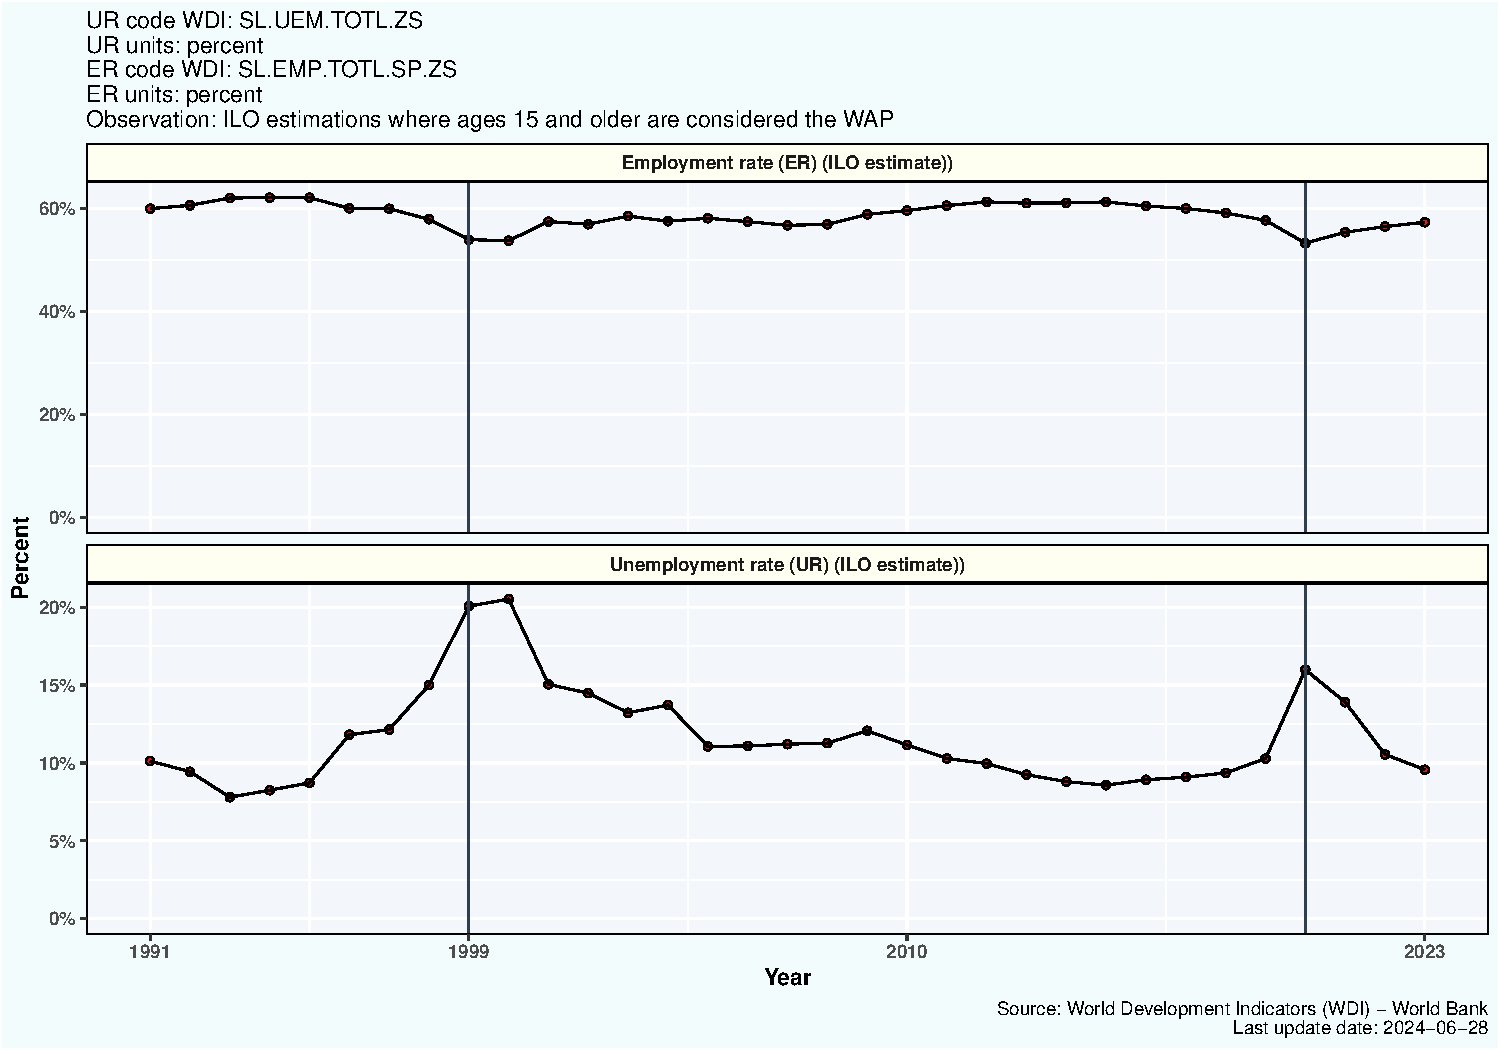
\includegraphics[width=0.85\textwidth,height=\textheight]{009_labor_market_files/figure-beamer/fig-ur-er-col-1.pdf}

}

\caption{\label{fig-ur-er-col}Annual Unemployment rate (UR) and
Employment rate (ER) in Colombia}

\end{figure}%
\end{frame}

\section{Labor demand}\label{labor-demand}

\begin{frame}{}
\phantomsection\label{section-7}
\begin{itemize}
\item
  The labor demand is the process by which the economy generates job
  vacancies
\item
  How companies decide how many workers to contract?

  \begin{itemize}
  \tightlist
  \item
    Demand of the products that offer by the company
  \item
    Wages (the price of labor)
  \item
    Labor regulation
  \item
    The costs of other inputs different form labor and used in
    production
  \item
    The technology used by companies
  \end{itemize}
\end{itemize}
\end{frame}

\begin{frame}{}
\phantomsection\label{section-8}
\begin{figure}

\centering{

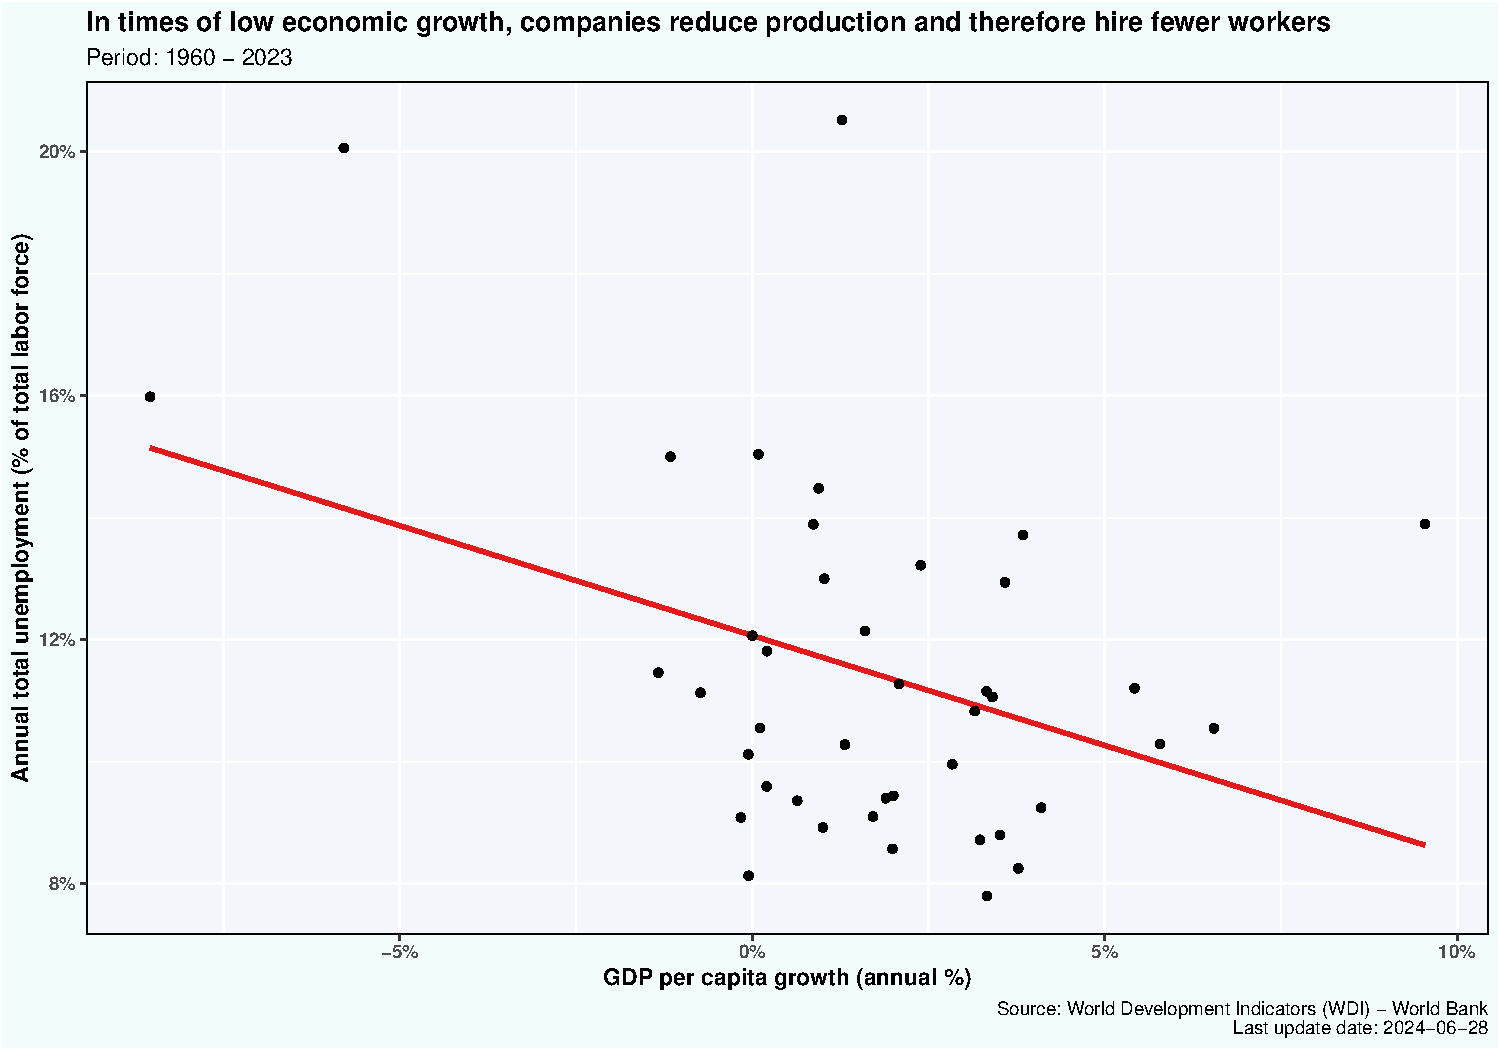
\includegraphics[width=0.85\textwidth,height=\textheight]{009_labor_market_files/figure-beamer/fig-economic-growth-ur-col-1.pdf}

}

\caption{\label{fig-economic-growth-ur-col}Economic growth vs
unemployment rate}

\end{figure}%
\end{frame}

\section{Wages}\label{wages}

\begin{frame}{}
\phantomsection\label{section-9}
\begin{figure}

\centering{

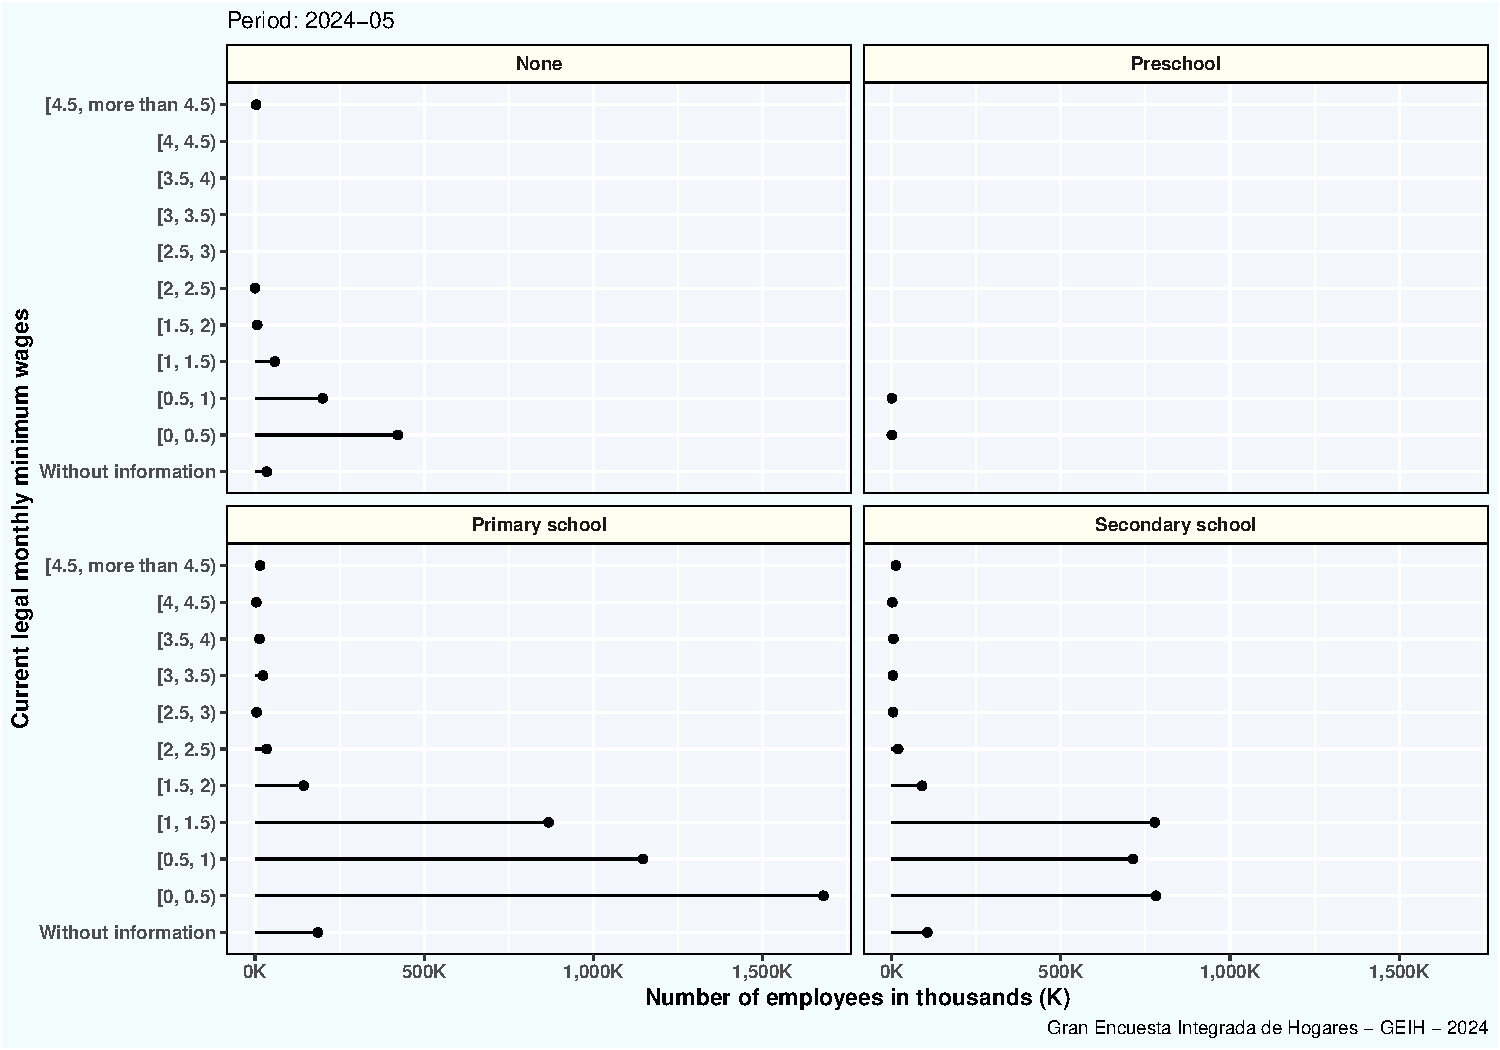
\includegraphics[width=0.85\textwidth,height=\textheight]{009_labor_market_files/figure-beamer/fig-income-education-level-1-1.pdf}

}

\caption{\label{fig-income-education-level-1}Employed population
according to last educational degree obtained and income bracket}

\end{figure}%
\end{frame}

\begin{frame}{}
\phantomsection\label{section-10}
\begin{figure}

\centering{

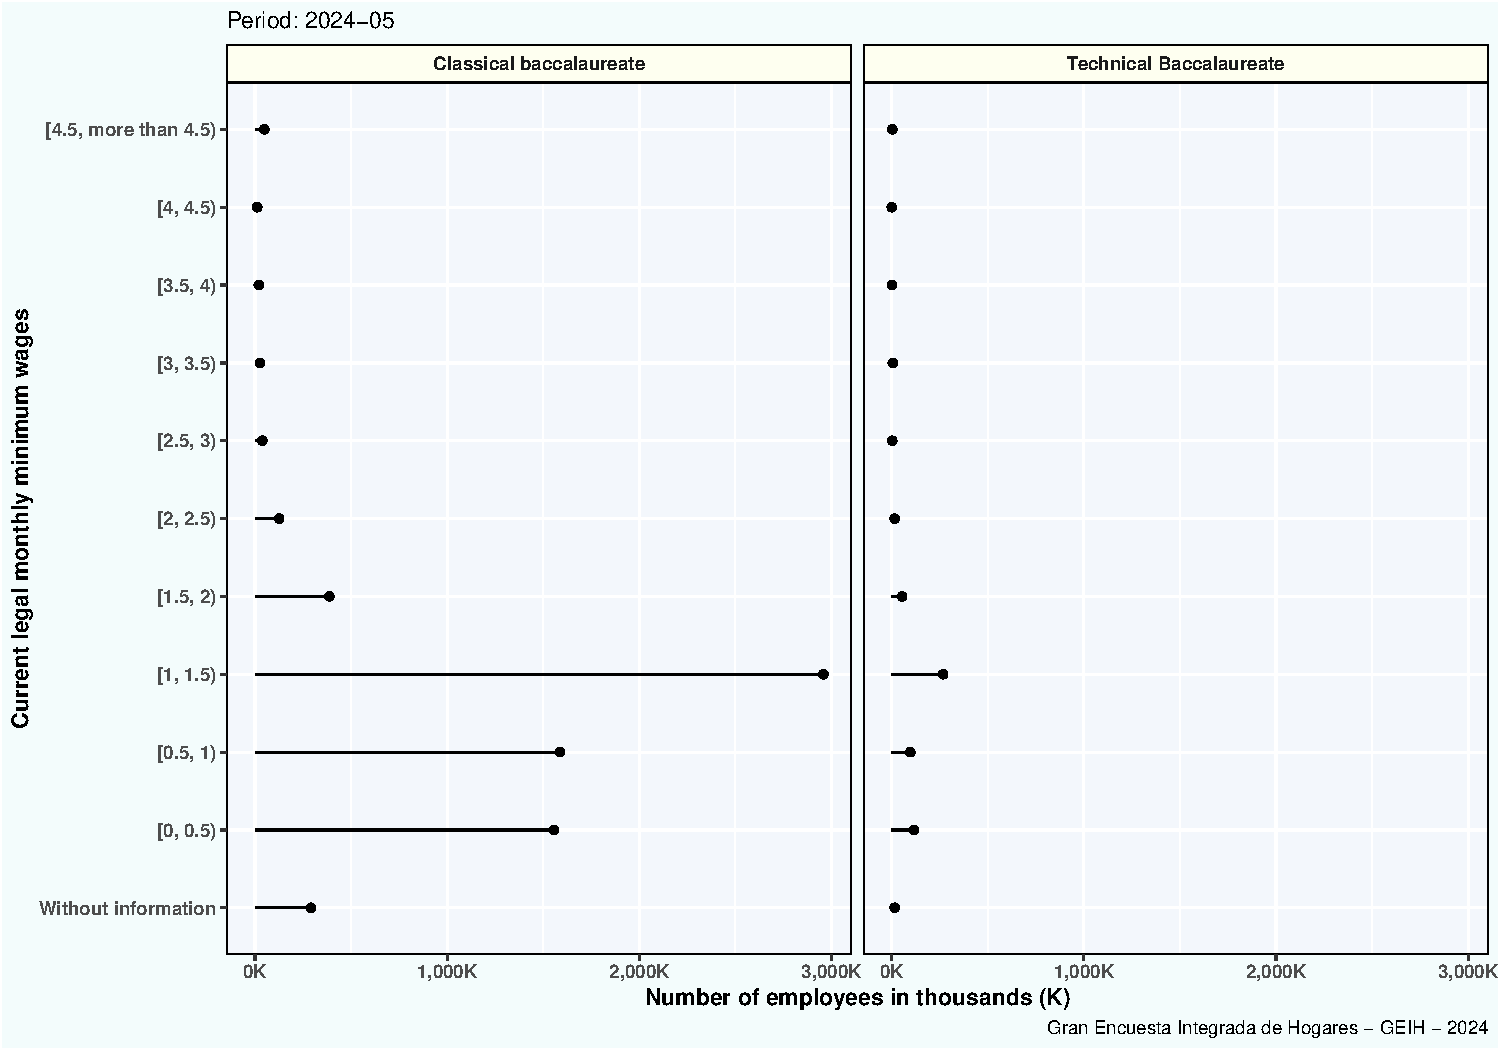
\includegraphics[width=0.85\textwidth,height=\textheight]{009_labor_market_files/figure-beamer/fig-income-education-level-2-1.pdf}

}

\caption{\label{fig-income-education-level-2}Employed population
according to last educational degree obtained and income bracket}

\end{figure}%
\end{frame}

\begin{frame}{}
\phantomsection\label{section-11}
\begin{figure}

\centering{

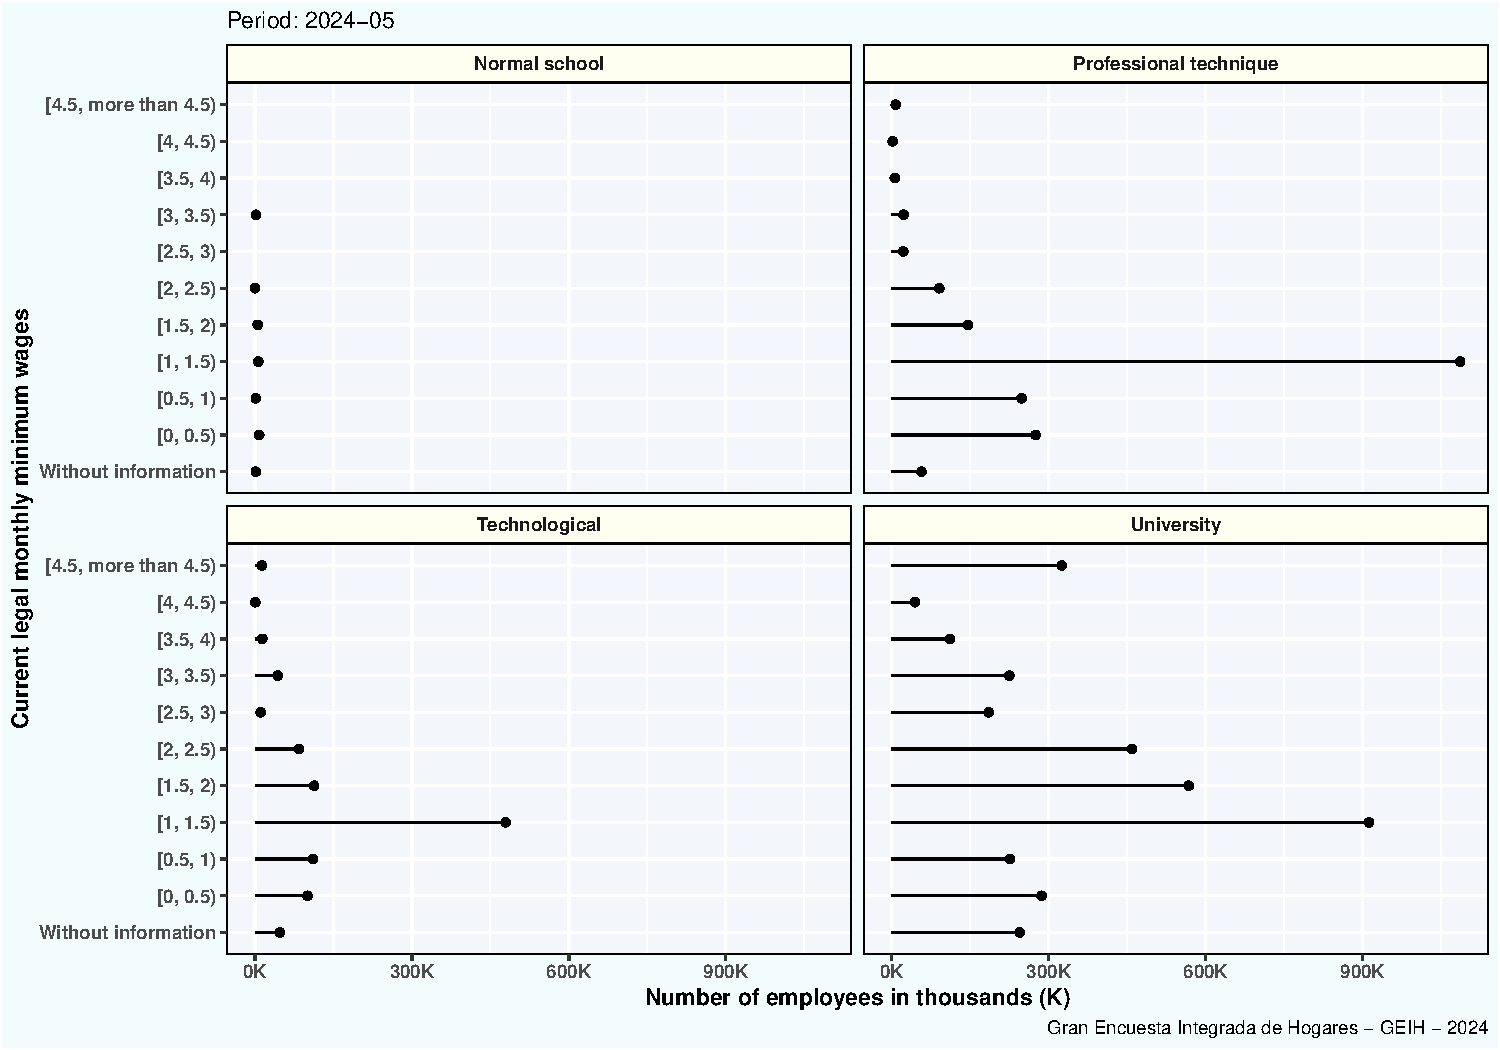
\includegraphics[width=0.85\textwidth,height=\textheight]{009_labor_market_files/figure-beamer/fig-income-education-level-3-1.pdf}

}

\caption{\label{fig-income-education-level-3}Employed population
according to last educational degree obtained and income bracket}

\end{figure}%
\end{frame}

\begin{frame}{}
\phantomsection\label{section-12}
\begin{figure}

\centering{

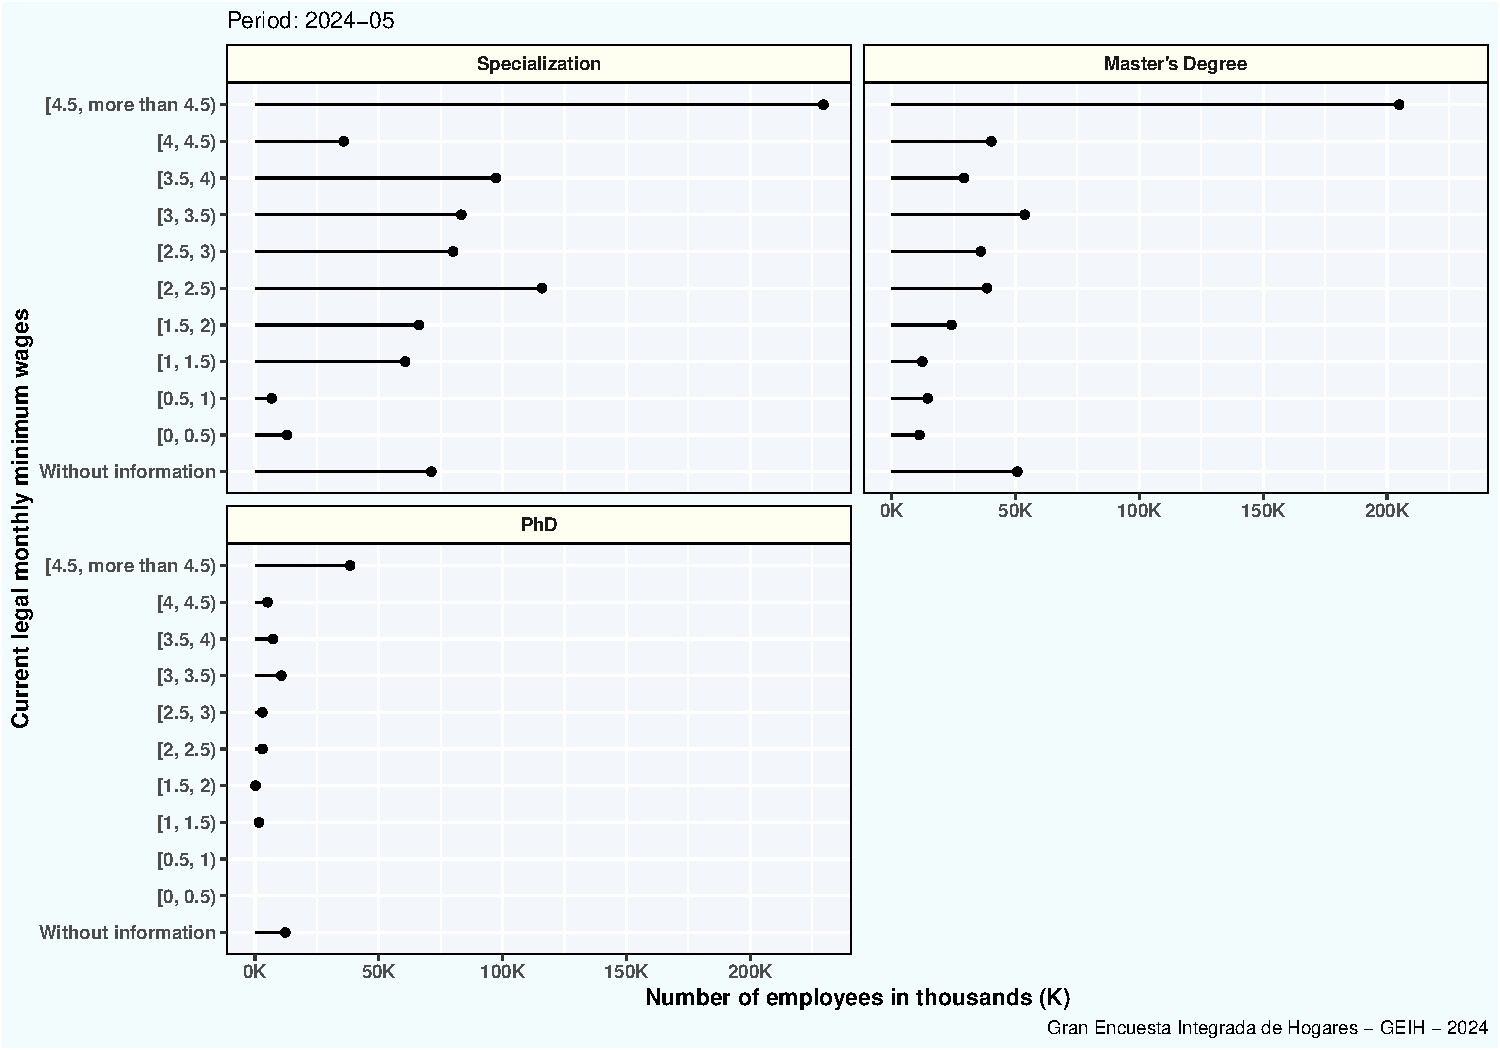
\includegraphics[width=0.85\textwidth,height=\textheight]{009_labor_market_files/figure-beamer/fig-income-education-level-4-1.pdf}

}

\caption{\label{fig-income-education-level-4}Employed population
according to last educational degree obtained and income bracket}

\end{figure}%
\end{frame}

\begin{frame}{}
\phantomsection\label{section-13}
\begin{itemize}
\item
  Mincer equation

  \begin{itemize}
  \item
    \(log_e(w_{it}) = log_e(w_o) + \beta_1Ed_{it} +  \beta_2Ex_{it} + \beta_2Ex_{it}^2 + \epsilon_{it}\)

    \begin{itemize}
    \tightlist
    \item
      \(log_e\): natural logarithm
    \item
      \(w_{it}\): wage of individual \(i\) in period \(t\)
    \item
      \(w_o\): wage without any level of education an experience
    \item
      \(\epsilon_{it}\): years of education of individual \(i\) in
      period \(t\)
    \item
      \(Ex_{it}\): potential experience of individual \(i\) in period
      \(t\) which is equal to the age minus the years of education minus
      six
    \item
      \(\epsilon_{it}\): are other components of individual \(i\) in
      period \(t\) that might affect the wage
    \end{itemize}
  \end{itemize}
\end{itemize}
\end{frame}

\section{Labor regulation}\label{labor-regulation}

\begin{frame}{}
\phantomsection\label{section-14}
\begin{itemize}
\item
  The labor regulation refers to:

  \begin{itemize}
  \tightlist
  \item
    The laws governing labor contracts
  \item
    Laws governing labor relations that empower unions to represent
    workers collectively
  \item
    Social security laws governing the response to social needs such as
    unemployment, maternity, old age, disability, death and sickness
  \end{itemize}
\end{itemize}
\end{frame}

\begin{frame}{}
\phantomsection\label{section-15}
\begin{itemize}
\item
  Resources

  \begin{itemize}
  \item
    \textbf{Calculadora Laboral - Mintrabajo}

    \begin{itemize}
    \tightlist
    \item
      \url{https://www.mintrabajo.gov.co/web/guest/inicio}
      \textgreater{} Atención al Ciudadano \textgreater{} Trámites y
      Servicios \textgreater{} Mi Calculadora
    \end{itemize}
  \end{itemize}
\end{itemize}
\end{frame}

\section{Economic environment and the
Company}\label{economic-environment-and-the-company}

\begin{frame}{}
\phantomsection\label{section-16}
\begin{figure}

\centering{

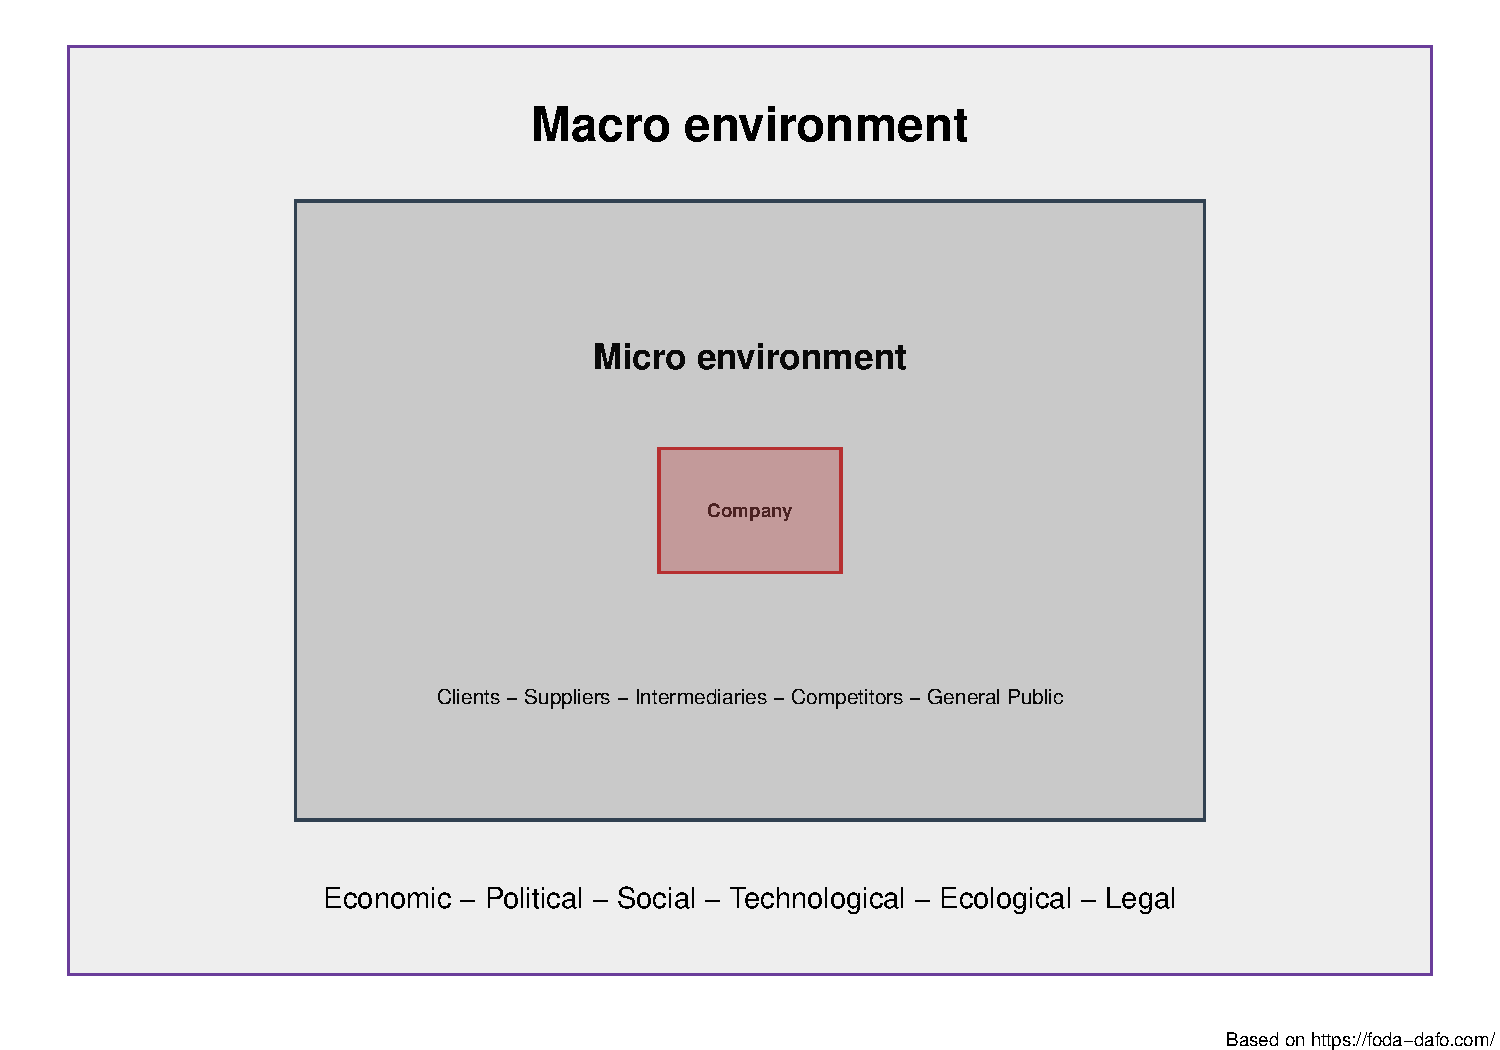
\includegraphics[width=0.85\textwidth,height=\textheight]{009_labor_market_files/figure-beamer/fig-econ-env-macro-1.pdf}

}

\caption{\label{fig-econ-env-macro}Set of economic factors and forces
that influence the development of an organization}

\end{figure}%
\end{frame}

\section{Acknowledgments}\label{acknowledgments}

\begin{frame}{}
\phantomsection\label{section-17}
\begin{itemize}
\item
  To my family that supports me
\item
  To the taxpayers of Colombia and the
  \href{https://www.umng.edu.co/estudiante}{\textbf{UMNG students}} who
  pay my salary
\item
  To the \href{https://www.business-science.io/}{\textbf{Business
  Science}} and \href{https://www.rfordatasci.com/}{\textbf{R4DS Online
  Learning}} communities where I learn
  \href{https://www.r-project.org/about.html}{\textbf{R}} and
  \href{https://www.python.org/about/}{\textbf{\(\pi\)-thon}}
\item
  To the \href{https://www.r-project.org/contributors.html}{\textbf{R
  Core Team}}, the creators of
  \href{https://rstudio.com/products/rstudio/}{\textbf{RStudio IDE}},
  \href{https://quarto.org/}{\textbf{Quarto}} and the authors and
  maintainers of the packages
  \href{https://CRAN.R-project.org/package=tidyverse}{\textbf{tidyverse}},
  \href{https://CRAN.R-project.org/package=tidyquant}{\textbf{tidyquant}},
  \href{https://CRAN.R-project.org/package=readxl}{\textbf{readxl}}, and
  \href{https://CRAN.R-project.org/package=tinytex}{\textbf{tinytex}}
  for allowing me to access these tools without paying for a license
\item
  To the \href{https://www.kernel.org/category/about.html}{\textbf{Linux
  kernel community}} for allowing me the possibility to use some
  \href{https://static.lwn.net/Distributions/}{\textbf{Linux
  distributions}} as my main
  \href{https://en.wikipedia.org/wiki/Operating_system}{\textbf{OS}}
  without paying for a license
\end{itemize}
\end{frame}

\section*{References}\label{references}
\addcontentsline{toc}{section}{References}

\begin{frame}[allowframebreaks]{References}
\phantomsection\label{refs}
\begin{CSLReferences}{1}{0}
\bibitem[\citeproctext]{ref-cardenas_introduccion_2020}
Cardenas, Mauricio. 2020. \emph{Introducción a La {Economía}
{Colombiana}}. 4th ed. Alfaomega.

\bibitem[\citeproctext]{ref-hussmanns_surveys_1990}
Hussmanns, Ralf, Farhad Mehran, and Vijaya Varmā. 1990. \emph{Surveys of
Economically Active Population, Employment, Unemployment, and
Underemployment: An {ILO} Manual on Concepts and Methods}. Geneva:
International Labour Office.
\url{https://www.ilo.org/global/statistics-and-databases/publications/WCMS_215885/lang--en/index.htm}.

\end{CSLReferences}
\end{frame}




\end{document}
